\section{Results: does EMD add anything?}
\label{sec:emd}

Figure~\ref{fig:emd} compares the EMD feature sets with band power. Hilbert band power from the IMFs comes close to Welch band power on held-out subjects: the mean difference runs from \N{c:hilb_min} to \N{c:hilb_max} across the three data sets (LDA, per channel, both normalizations), and none is significant after Holm's correction, though no equivalence test was run. Within subjects on the two motor-imagery data sets, it is lower on average (\N{pt:eeg_mmi:within:none:lda:F3_ch:F1_ch} on EEG MMI and \N{pt:bci_civ_2a:within:none:lda:F3_ch:F1_ch} on BCI IV 2a, where \N{pd:bci_civ_2a:within:none:lda:F3_ch:F1_ch:lower} of 9 subjects are lower). The IMF features themselves, the first four IMFs summarized by log variance, mean absolute instantaneous frequency, and entropy, score below band power: \N{c:imfbp_min} to \N{c:imfbp_max} on held-out subjects (LDA, per channel, standardized; \N{c:imfbp_none_min} to \N{c:imfbp_none_max} unstandardized), with none significant after correction. Within EEG MMI subjects, the gap is \N{pt:eeg_mmi:within:none:lda:F2_ch:F1_ch} (Holm $p$ \N{pt:eeg_mmi:within:none:lda:F2_ch:F1_ch:ph}), but that comparison partly reflects dimensionality: with channels kept separate, the IMF set has 36 features against band power's 15, and each within-subject fold trains on about 36 windows. The IMF set's own within-subject mean, \N{sm:eeg_mmi:F2_ch:lda:within:none}, is below its held-out mean, \N{sm:eeg_mmi:F2_ch:lda:heldout:none} unstandardized, which suggests too many features for too few windows rather than missing information, though the study does not vary the number of features. The held-out comparison is the fairer one.

\begin{figure}[t]
\centering
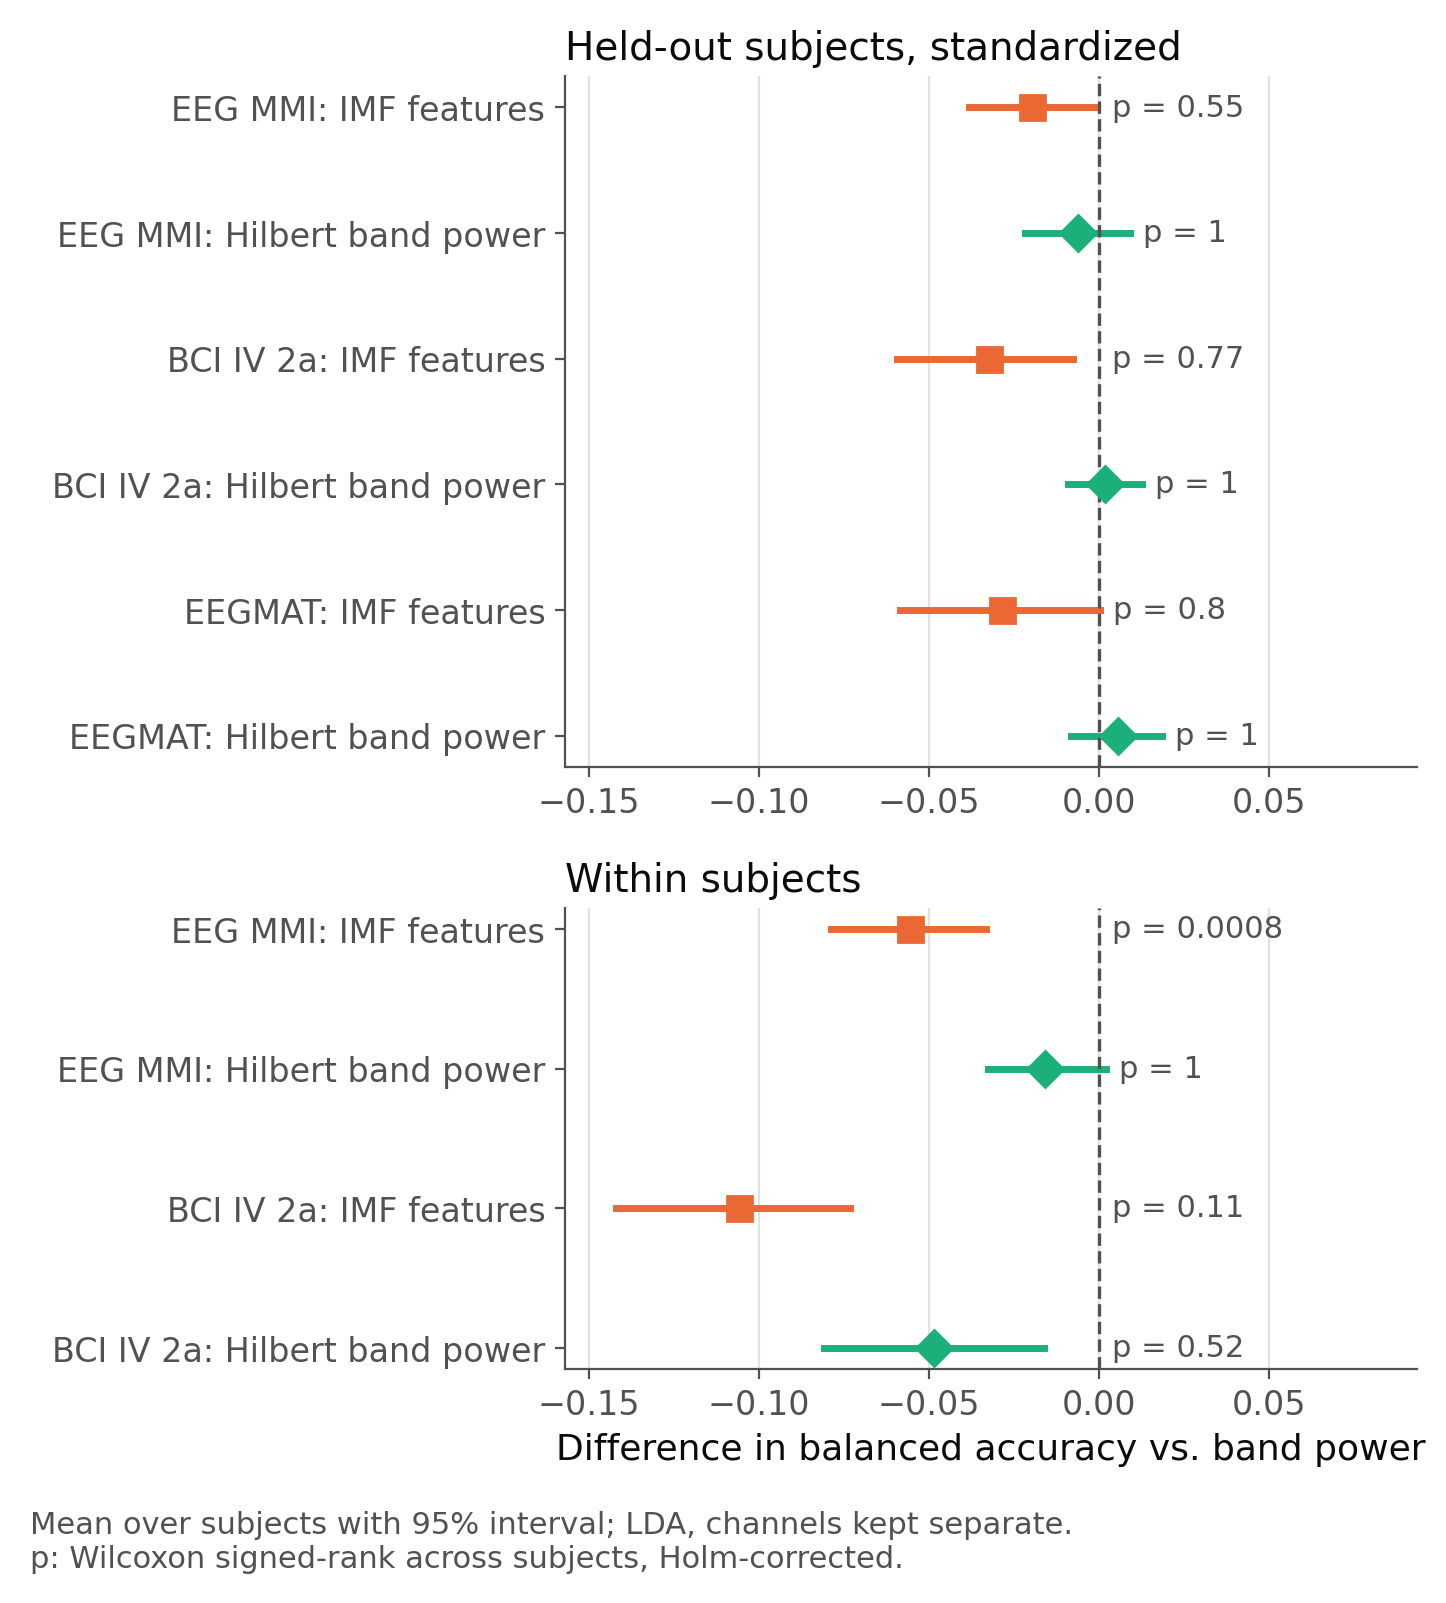
\includegraphics[width=\columnwidth]{../results/study/figures/fig3_emd_vs_bandpower.png}
\caption{Per-channel IMF features and Hilbert band power minus band power, LDA, with Holm-adjusted $p$: on held-out subjects with features standardized within each subject (top), and within subjects for EEG MMI and BCI IV 2a (bottom; EEGMAT is left out there).}
\label{fig:emd}
\end{figure}

Over all \N{c:emd_total} comparisons of an EMD feature set against band power (averaged and per channel, three classifiers, three subject-based evaluations (within subjects, and held out as is and standardized), and four data set variants, the fourth being BCI late), \N{c:emd_above} intervals lie above zero (the largest difference is \N{c:emd_above_max}), \N{c:emd_below} lie below, and \N{c:emd_holm} pass Holm's correction, both against EMD and both within subjects (the per-channel IMF features, with LDA on EEG MMI and with Euclidean KNN on EEGMAT). The late BCI IV 2a window changes little: band power per channel with LDA scores \N{sm:bci_civ_2a_late:F1_ch:lda:within:none} against \N{sm:bci_civ_2a:F1_ch:lda:within:none} within subjects, and \N{sm:bci_civ_2a_late:F1_ch:lda:heldout:subject} against \N{sm:bci_civ_2a:F1_ch:lda:heldout:subject} on held-out subjects (standardized; \N{sm:bci_civ_2a_late:F1_ch:lda:heldout:none} against \N{sm:bci_civ_2a:F1_ch:lda:heldout:none} unstandardized). Of the \N{c:lda_ch_heldout_total} held-out LDA comparisons with channels kept separate, no interval favors EMD and \N{c:lda_ch_heldout_bp_better} favor band power. A likely reason, offered as an interpretation that no result here tests, is that with sensible IMFs the Hilbert band power of the IMFs measures the same power in the same bands as a filter bank.
